\subsection{System Architecture and Data Model}

This section presents multiple architectural views of the LiftDrop platform, highlighting how its components interact and how its data model is structured. Each diagram focuses on a different conceptual layer of the system, from user roles and sessions to request fulfillment and geolocation modeling.

\subsubsection{High-Level System Architecture}

Figure~\ref{fig:high-level-Overview} shows the overall system architecture. It illustrates the interaction between the Android mobile application and backend services responsible for order assignment, real-time messaging, authentication, and location tracking.

\vspace{5mm}

\begin{figure}[H]
    \centering
    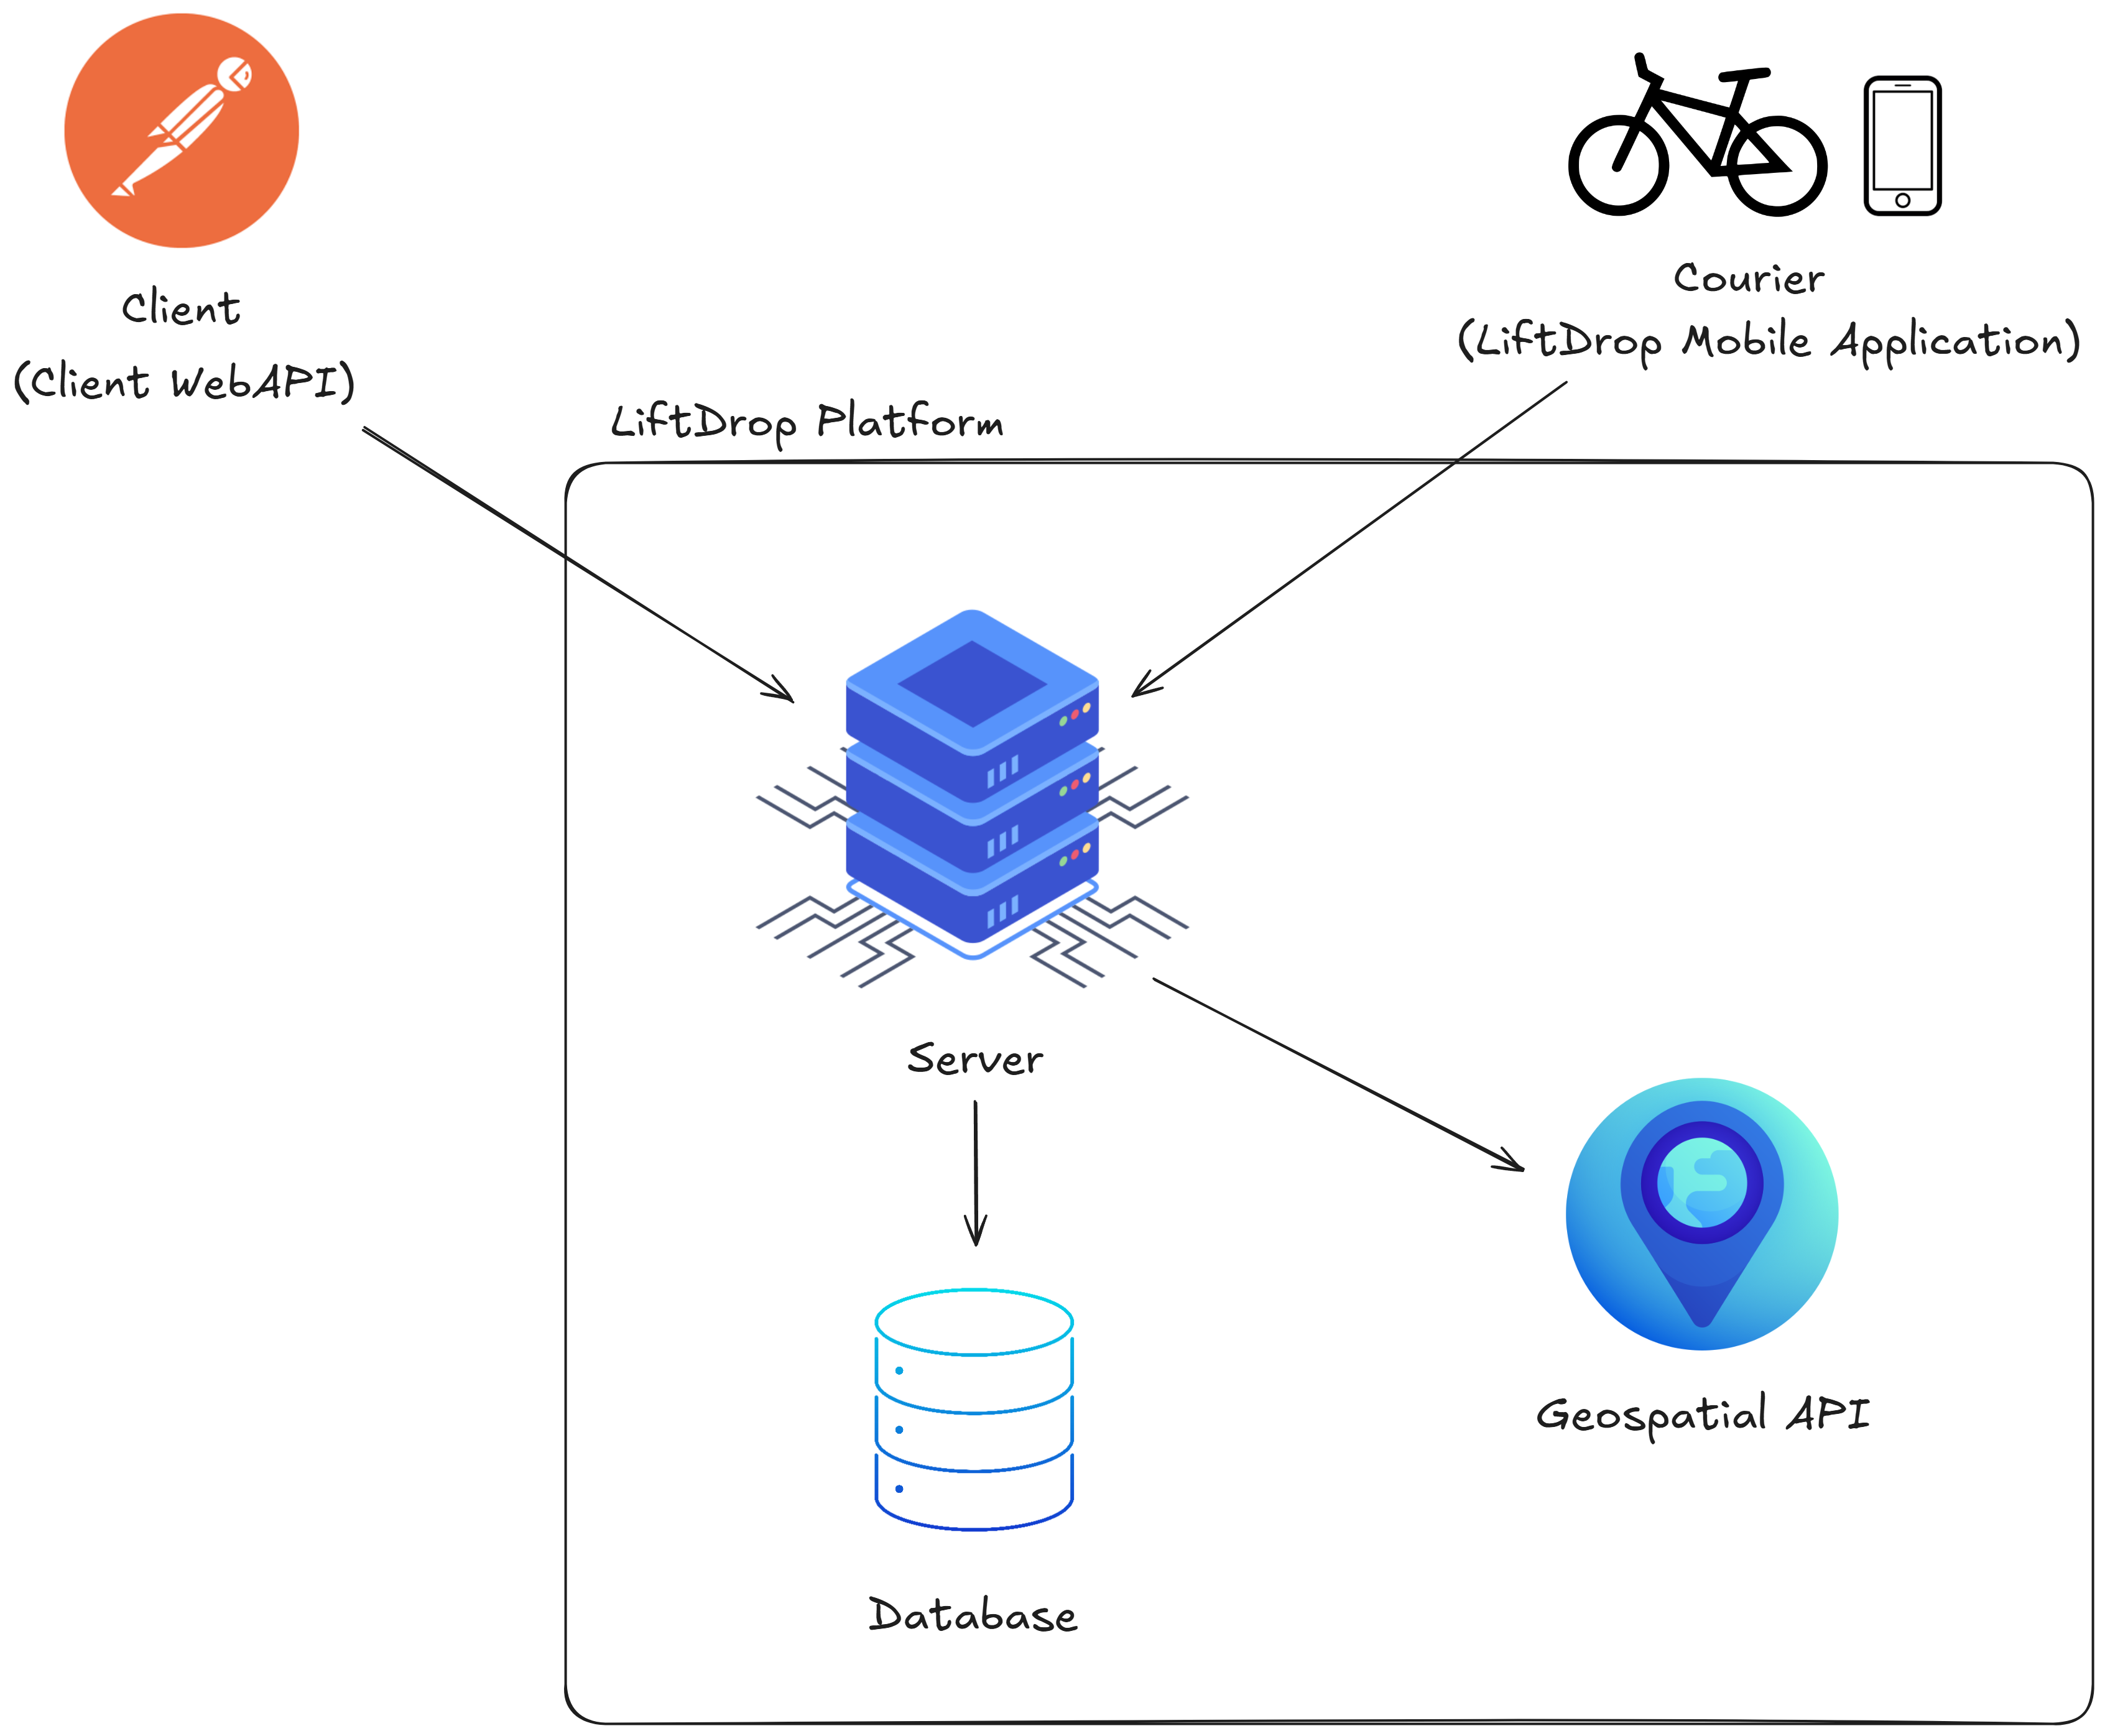
\includegraphics[width=0.82\textwidth]{images/LiftDrop_High_level_view.png}
    \caption{High-level overview of the LiftDrop system architecture}
    \label{fig:high-level-Overview}
\end{figure}

\newpage

\subsubsection{User and Role Hierarchy}

This diagram illustrates how the abstract \texttt{User} entity is specialized into the \texttt{Client} and \texttt{Courier} roles. It also shows how sessions are managed on a per-user basis for secure authentication.

\begin{figure}[H]
    \centering
    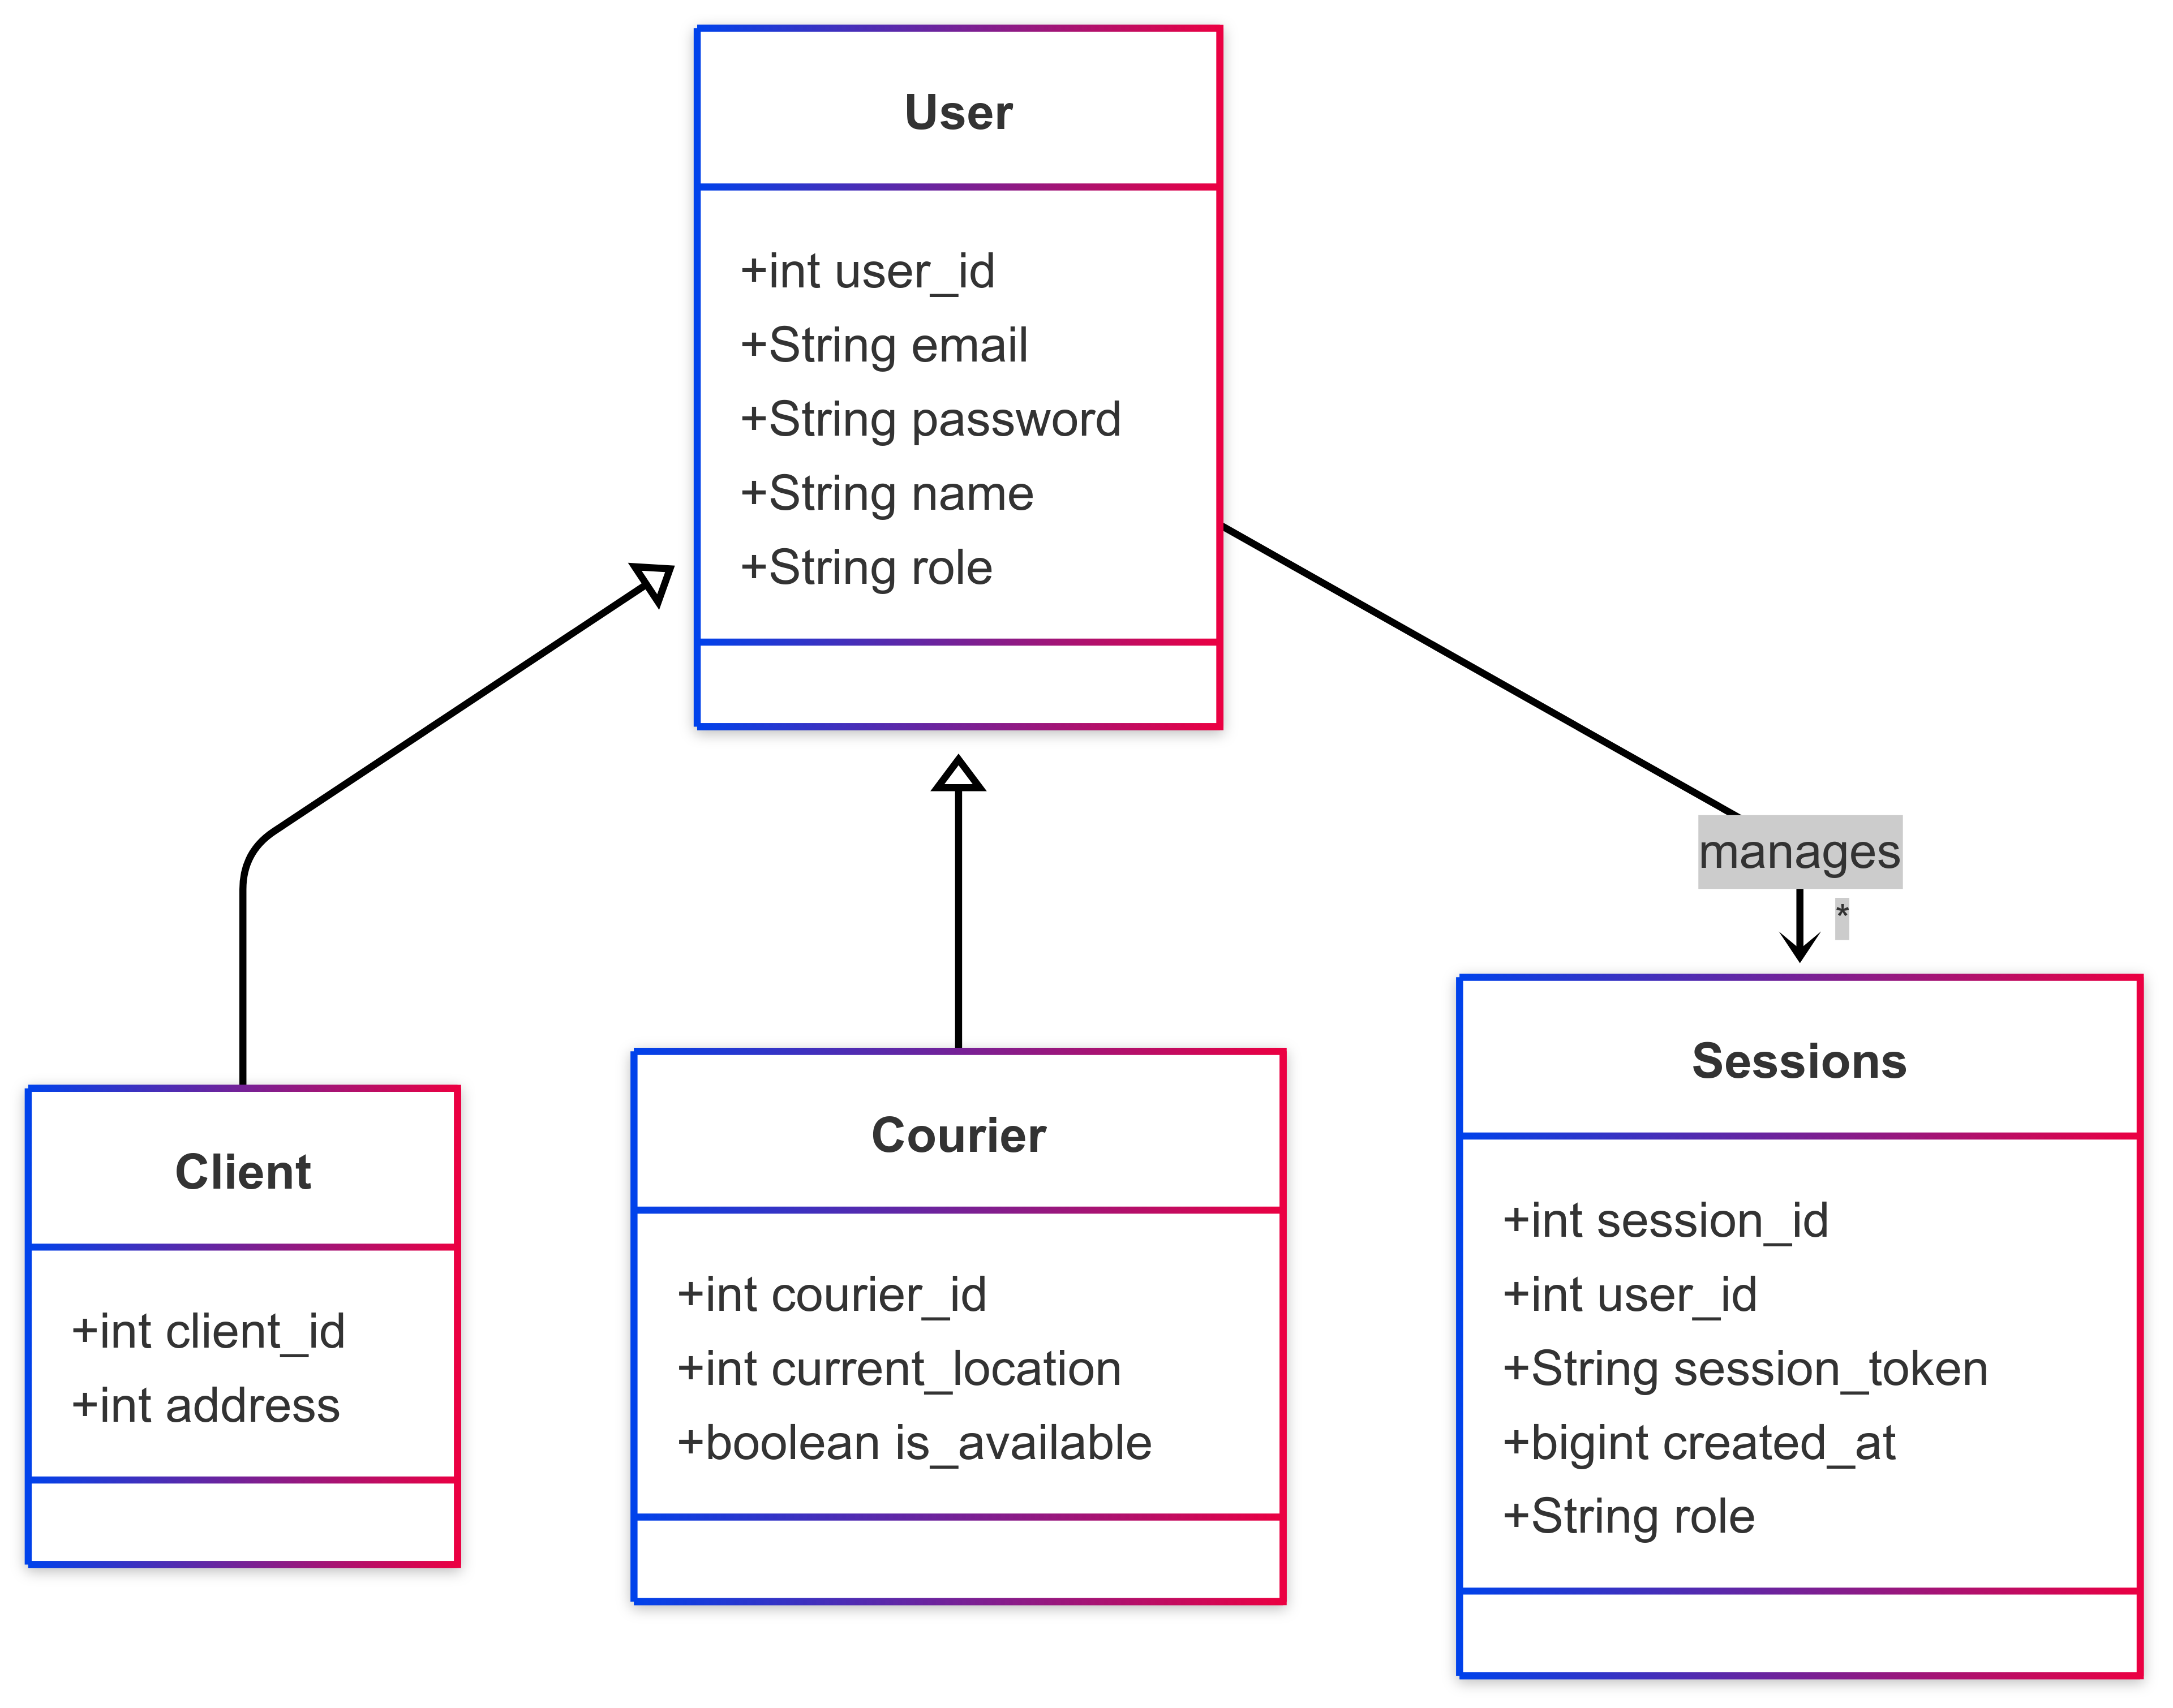
\includegraphics[width=0.60\textwidth]{images/classDiagrams/user_role_hierarchy.png}
    \caption{User roles and session relationships}
\end{figure}

\newpage

\subsubsection{Request and Delivery Lifecycle}

This model depicts the lifecycle of a delivery—from creation of a request by a client, through courier assignment, to delivery completion and rating. It reflects how entities such as \texttt{Request}, \texttt{Delivery}, and \texttt{CourierRating} are interlinked throughout the delivery flow.

\begin{figure}[H]
    \centering
    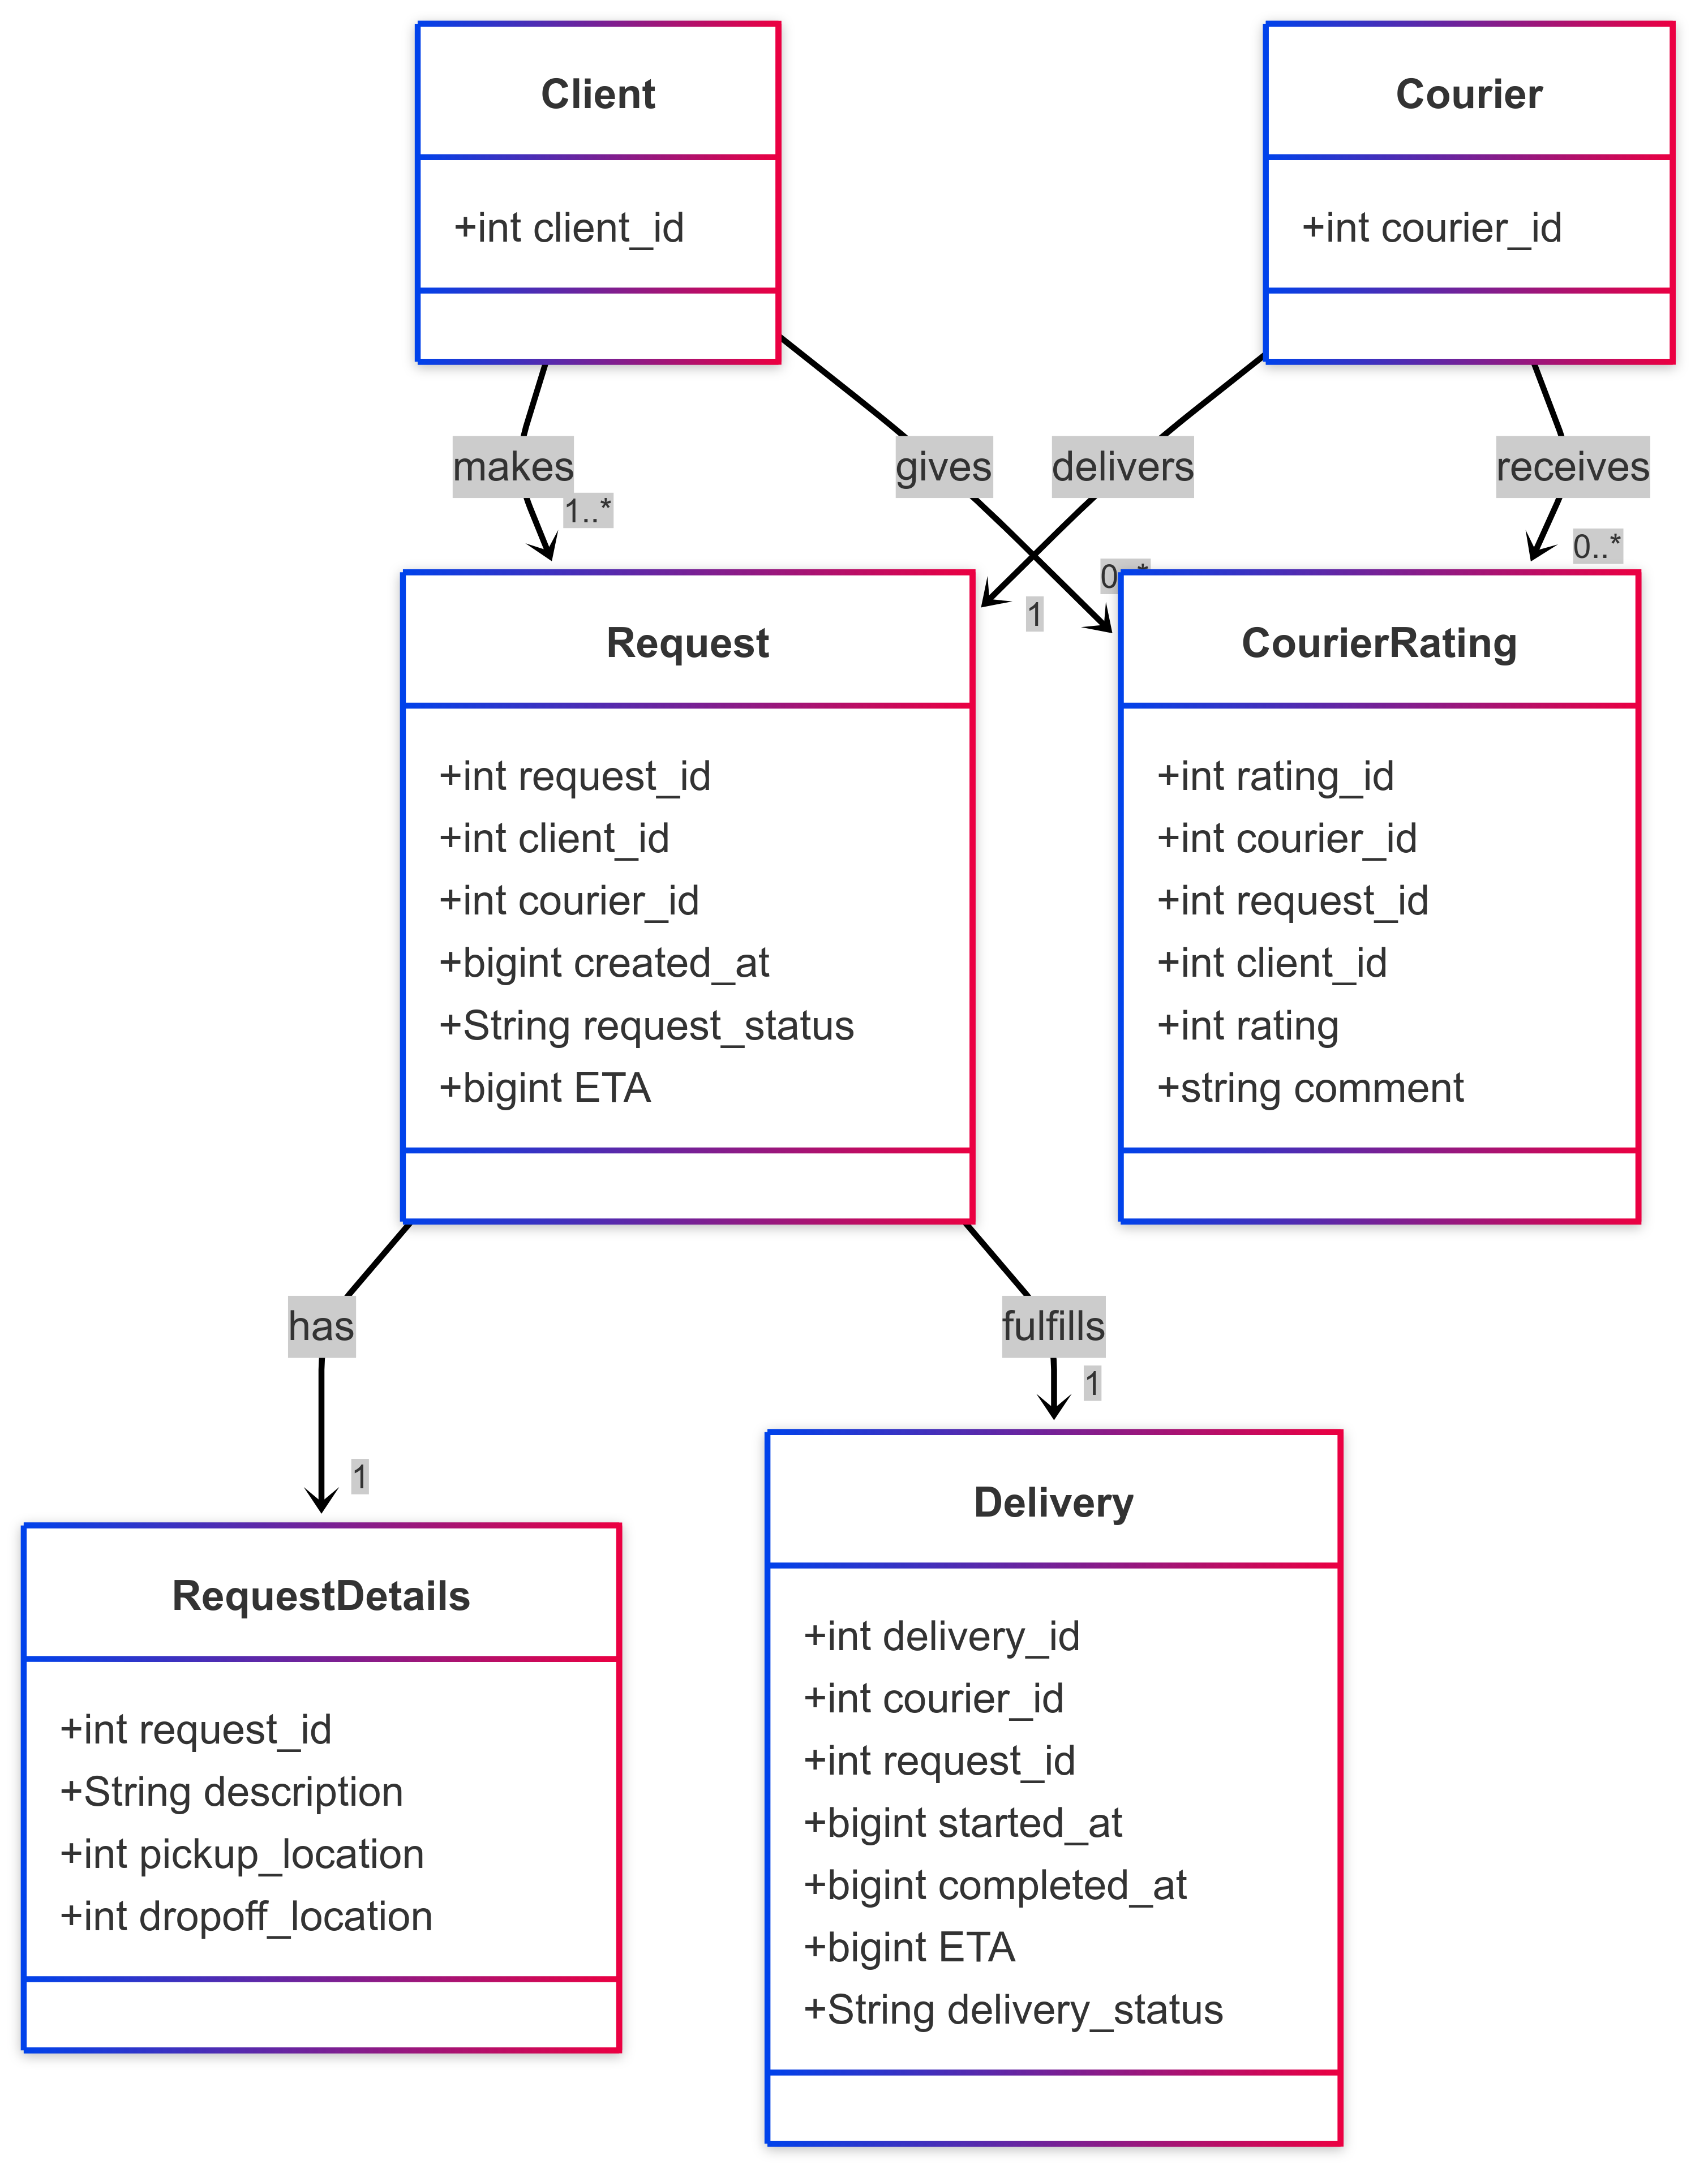
\includegraphics[width=0.65\textwidth]{images/classDiagrams/request_lifecycle.png}
    \caption{Request and Delivery lifecycle}
\end{figure}

\newpage

\subsubsection{Location and Address Modeling}

This view focuses on how real-world geographic data is modeled within the platform. It shows the relationship between generalized \texttt{Location} entities and their specializations—\texttt{PickupSpot} and \texttt{DropOffSpot}—as well as how these relate to physical addresses.

\begin{figure}[H]
    \centering
    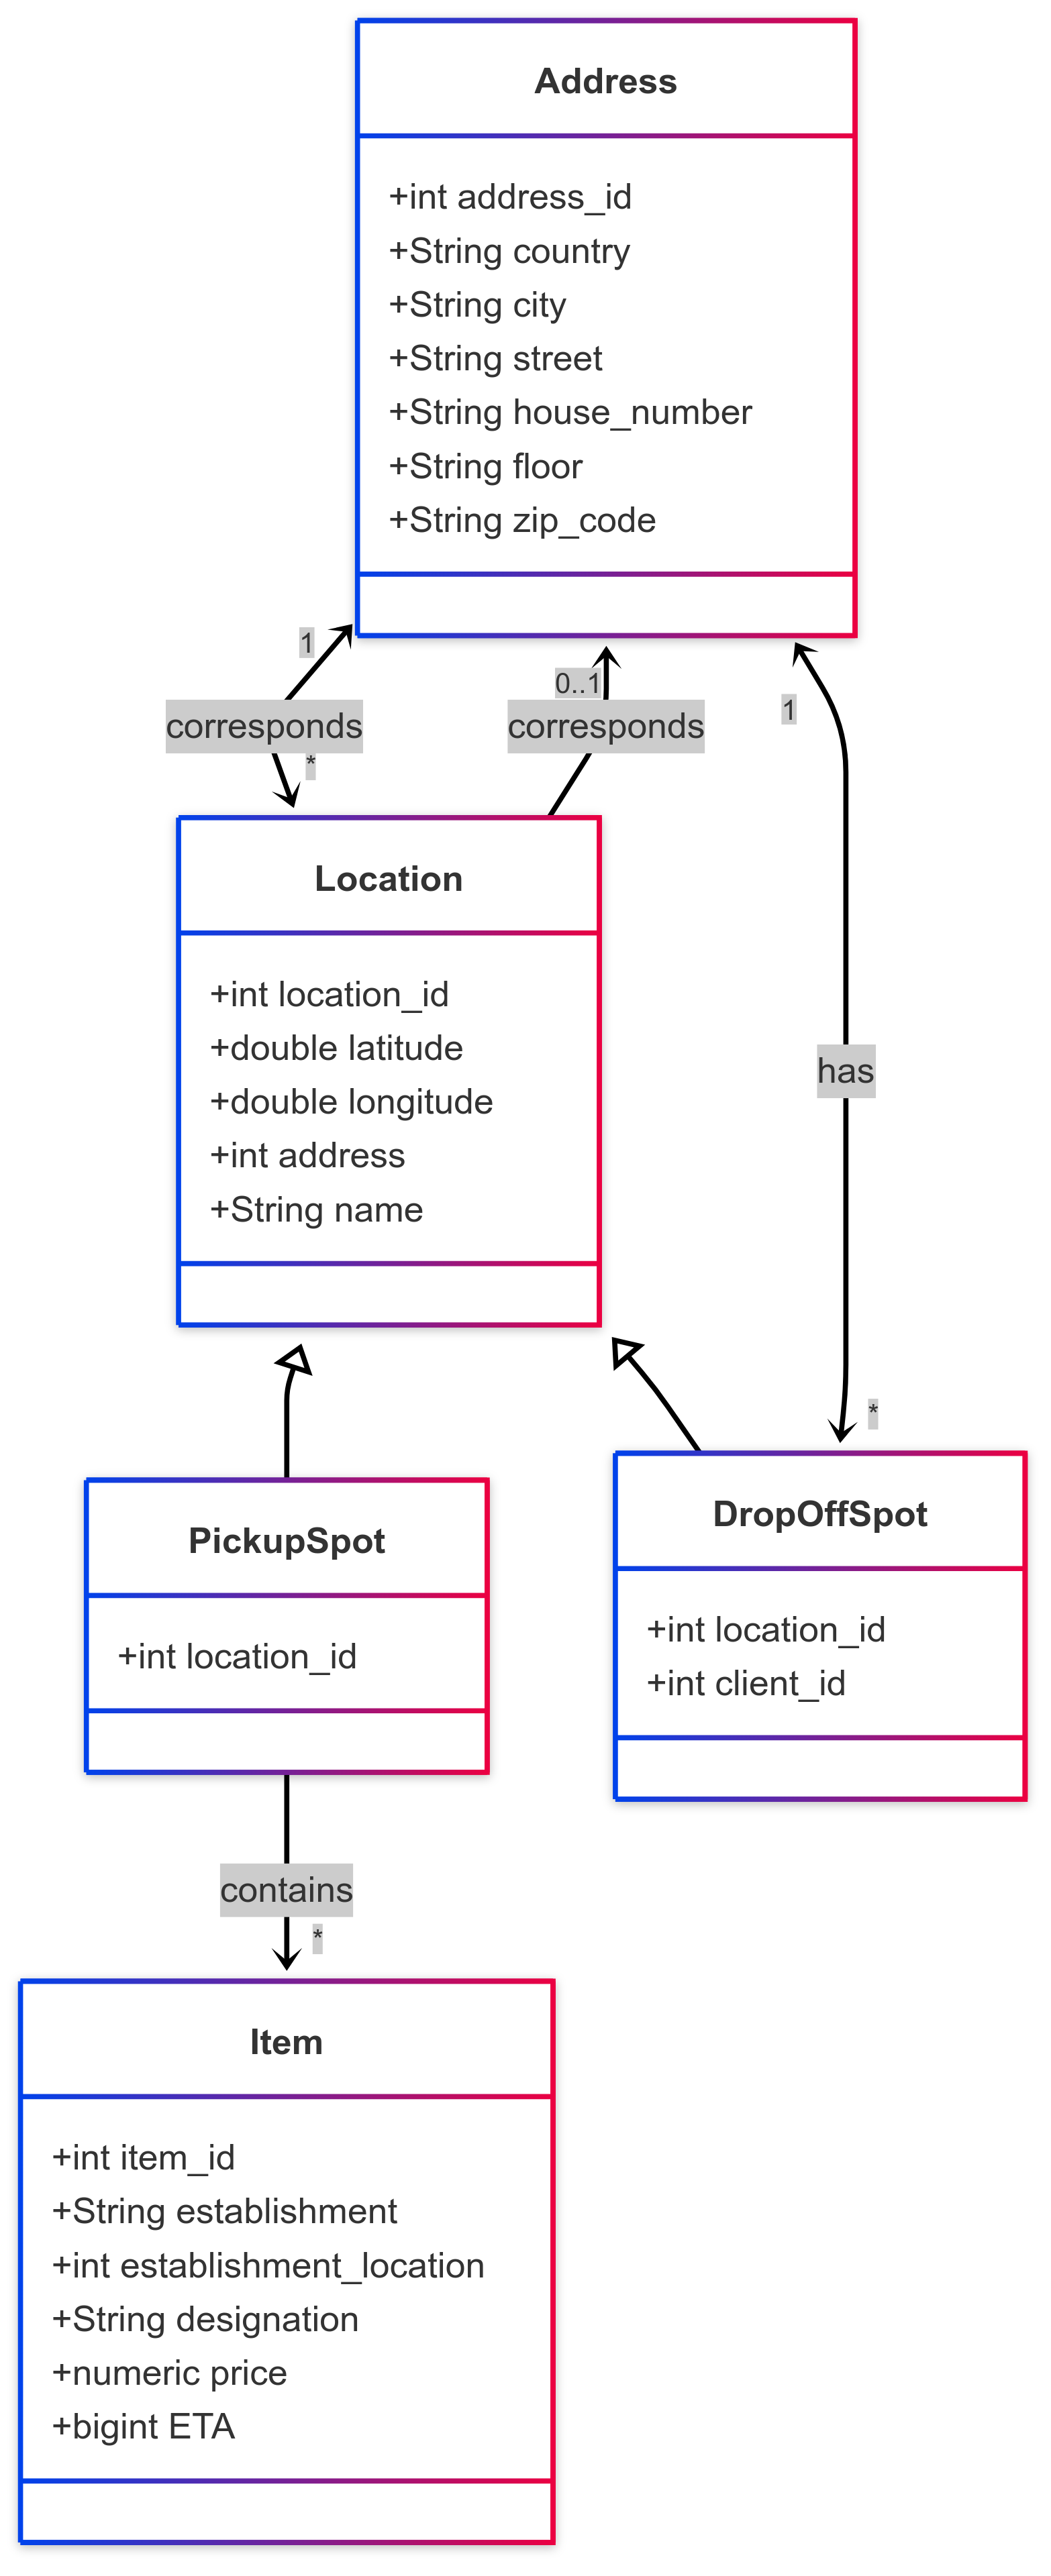
\includegraphics[width=0.45\textwidth]{images/classDiagrams/location_address_model.png}
    \caption{Location and Address structure}
\end{figure}

\bigskip

\noindent For a complete view of the system’s data model, including all class relationships and fields, refer to the full class diagram provided in Appendix~\ref{appendix:full-class-diagram}.
